\documentclass{article}
\usepackage{graphicx}
\usepackage{amsmath}
\usepackage{fancyhdr}
\usepackage[margin=1in]{geometry}
\usepackage{comment}
\usepackage{placeins}
\usepackage{parskip}
\usepackage{subcaption}
\usepackage{appendix}
\usepackage{soul}
\usepackage{comment}
\usepackage[hidelinks]{hyperref}
\usepackage{matlab-prettifier}
\usepackage{minted}
\usepackage{enumitem}
\usepackage{float}

\pagestyle{fancy}
\fancyhf{} % Clear header/footer settings
\rhead{\thepage} % Page number on the right in the header
\lhead{ASE375 Lab Report 2} % Your lab report title on the left

\begin{document}

\begin{titlepage}
  \centering
  
\includegraphics[width=10cm]{ase-logo-formal.png}  % Adjust the width as needed
  \vspace{1cm}  % Add some vertical space
 
  \Large \textbf{ASE 375 Electromechanical Systems}\\
  \large \textbf{Section 14115}\\
  \vspace{0.5cm}
  \textbf{Monday: 3:00 - 6:00 pm}\\
 
  \vspace{1cm}
 
  \hrule
  \vspace{0.5cm}
 
  \Huge \textbf{Report 2:\\
  Temperature Sensor Measurements}\\
  \Huge \textbf{}\\
 
  \vspace{0.5cm}
  \hrule
 
  \vspace{1cm}
 
  \normalsize \textbf{Andrew Doty, Andres Suniaga, Dennis Hom}\\
  \normalsize \textbf{Due Date: 02/12/2024}
 
\end{titlepage}
\newpage

\tableofcontents
\thispagestyle{empty}
\newpage

\section{Introduction}
This experiment consisted of measuring temperature with three different sensors: a Thermocouple, Thermistor, and an Integrated Circuit Temperature sensor. Data collection was made possible through a Data Acquisition (DAQ) system used to process the different temperature measurements in LabVIEW, a graphical interface that modeled the temperature sensors' measurements in real-time. 

The purpose of this experiment was to learn how to simulate our data through LabVIEW along with observing and understanding the behaviour of the three temperature sensors in different environments: $(1)$ at room temperature, $(2)$ in water near freezing conditions, and $(3)$ in water closer to boiling conditions. 

\section{Equipment}
The equipment used in this experiment include the following:  

K-type Thermocouple:  Temperature sensor with two different metals joined together at one end.  A K-type thermocouple uses Chromel-Alumel metals.  It will be connected to the DAQ via the NI 9211 thermocouple input module.  

SA1-TH Series Thermistor:  Temperature sensor that measures electrical resistance as a response to a change in temperature.  It is connected to the NI 9215 via breadboard in its own circuit with $1\text{k}\;\Omega$ resistor.
\begin{figure}[H]
    \centering
    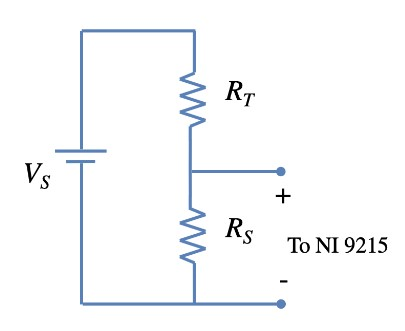
\includegraphics[width=0.25\textwidth]{Lab 2/lab2images/thermistor_circuit.jpg}
    \caption{Thermistor Circuit}
\end{figure}

TMP36 Temperature Sensor: Analog low voltage sensor.  It is connected to the NI 9215 via the breadboard.  

Breadboard: a reusable solderless prototyping board used for building electronic circuits. Components are inserted into interconnected rows and columns of holes, allowing for easy and temporary assembly of circuits for testing and experimentation.

Circuit Components:  various length male-to-male jumper wires, $1\text{k}\;\Omega$ resistor, 5V power supply.

DAQ:  Data Aquisition system that digitizes analog information into "bins" for a computer.  The specific DAQ had two units, the NI 9215 and NI 9211.  Specific Datasheets for each are included in the appendices.  

Thermometer:  Regular mercury thermometer, using change in volume as a response to a change in temperature.  Used to measure true temperature with 0.5 degrees least count.  

Water:  Access to water at two temperatures, near boiling, and ice cold. 


\section{Procedure}
\begin{figure}[H]
\centering
\includegraphics[width=0.5\textwidth, angle = -90]{Lab 2/lab2images/circuit_board_mug_and_sensors.jpg}
\caption{Temperature Sensors, Water mug, and Breadboard circuit}
\end{figure}

\section{Data Processing}
\subsubsection*{Variables}
\begin{enumerate}[label = \roman*.]
    \item \(N = \) Number of Samples
    \item \(f_{s} = \) Sampling Frequency, $s^{-1}$
    \item \(\Delta t_{s} = \) Sampling Interval, $s$
    \item \(\gamma = \) Confidence Level, \%
    \item \(R_{S} = \) Sensor Resistance, Ohms = $\Omega$ (In this experiment it will be $1\text{k}\Omega$)
    \item \(V_{S} = \) Source voltage, Volts = $V$ ($5\;V$ for this experiment)
    \item \(R_{T} = \) Themistor resistance, $\Omega$
\end{enumerate}

\subsubsection*{Equations}
\begin{enumerate}[label = \Roman*.]
    \item Sample Mean: \(\bar{x} = \dfrac{1}{N}\displaystyle\sum_{i=1}^{N} x_{i}\) 
    \item Standard Deviation of finite $N$, normalized by $N-1$: \(S_{x} = \sqrt{\displaystyle\sum_{i=1}^{N} \dfrac{(x_{i} - \bar{x})^{2}}{N-1}}\)
    \item Standard Deviation of the Mean: \(\dfrac{S_{x}}{\sqrt{N}}\)
    \item Measurement w/ Confidence Interval: \(\bar{x} \pm t_{stat}\cdot \dfrac{S_{x}}{\sqrt{N}}\)
    \item \textit{Steinhart-Hart Relation}: \(\dfrac{1}{T} = A + B\cdot ln(R_{T}) + C\cdot (ln(R_{T}))^{3}\)
\end{enumerate}
 
\begin{figure}[H]
\centering
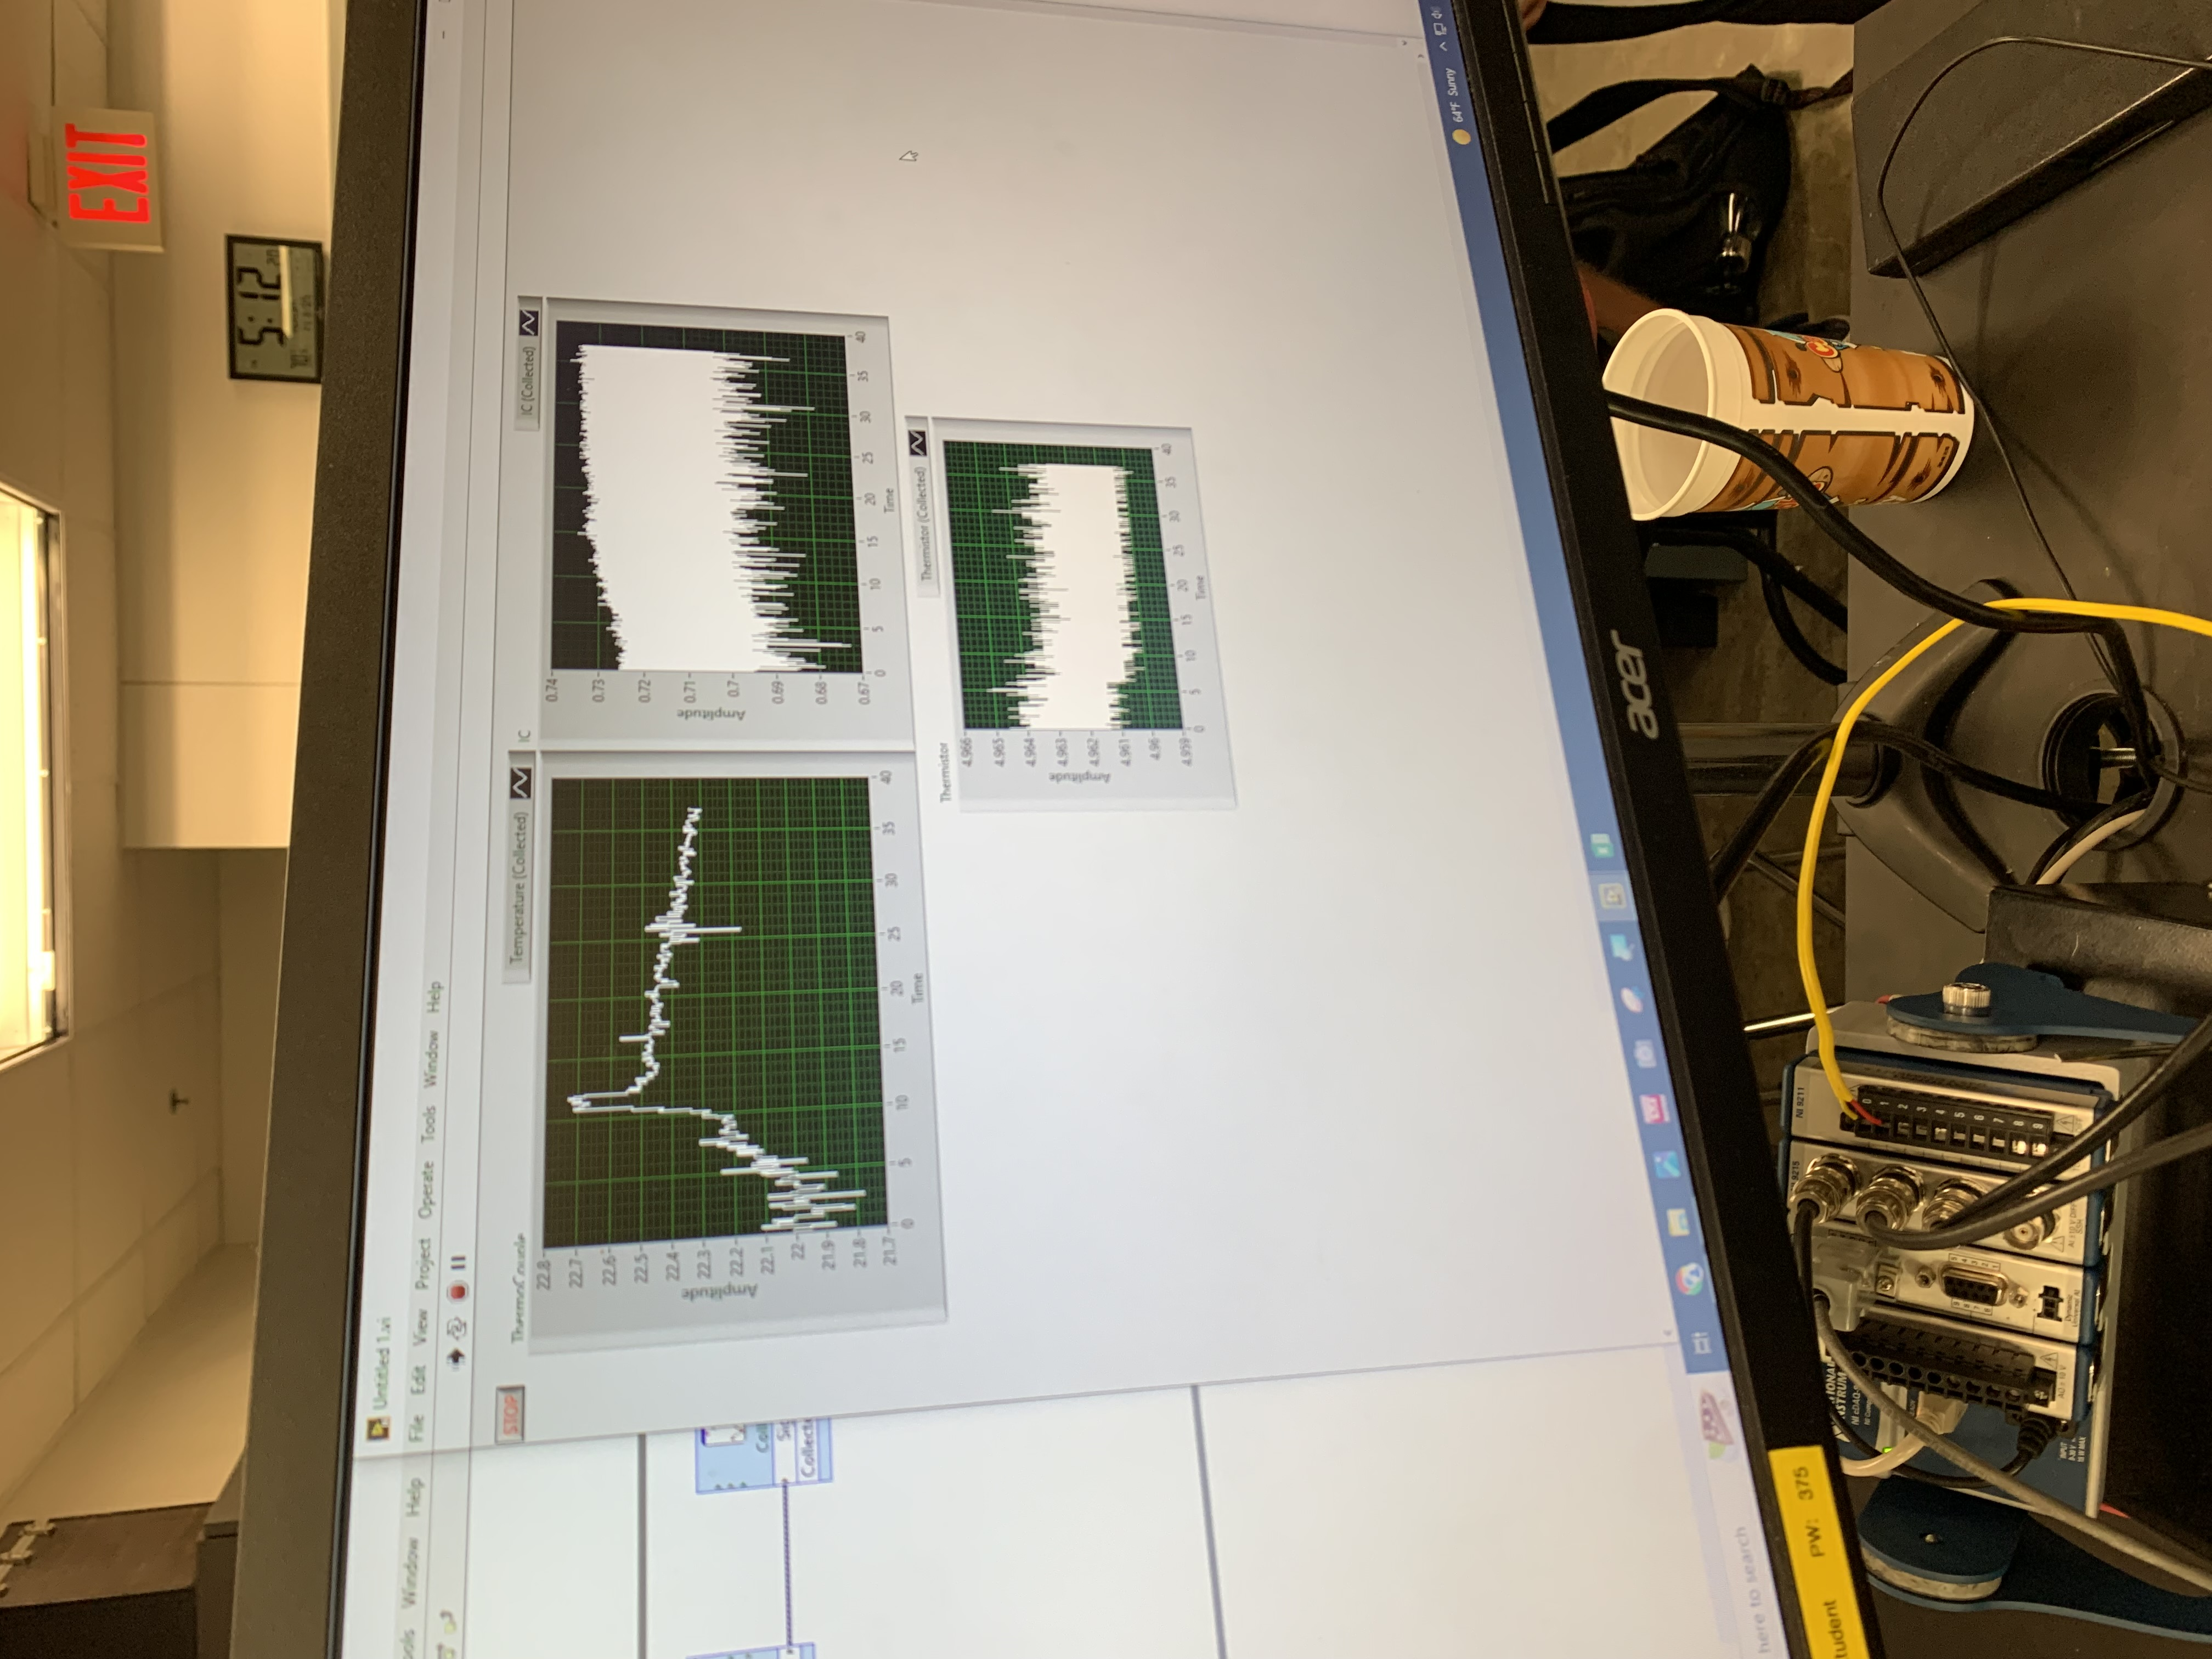
\includegraphics[width=0.5\textwidth, angle = -90]{Lab 2/lab2images/labview_plots.jpg}
\caption{Plotting data on LabVIEW}
\end{figure}

\subsection{Part 1: Ambient Temperature}
In Part 1 of the experiment we take measurements of the laboratory room temperature using each of the three sensors: thermocouple, thermistor, and IC TMP36. The data displayed below shows the temperature sensors at work for $1$ minute of sampling at $f_{s} = 1000\; s^{-1}$. This means $\Delta t_{s} = (f_{s}\cdot 60)^{-1} = 1.6667\times10^{-5}\; \text{minutes}$.

\begin{figure}[H]
    \centering
    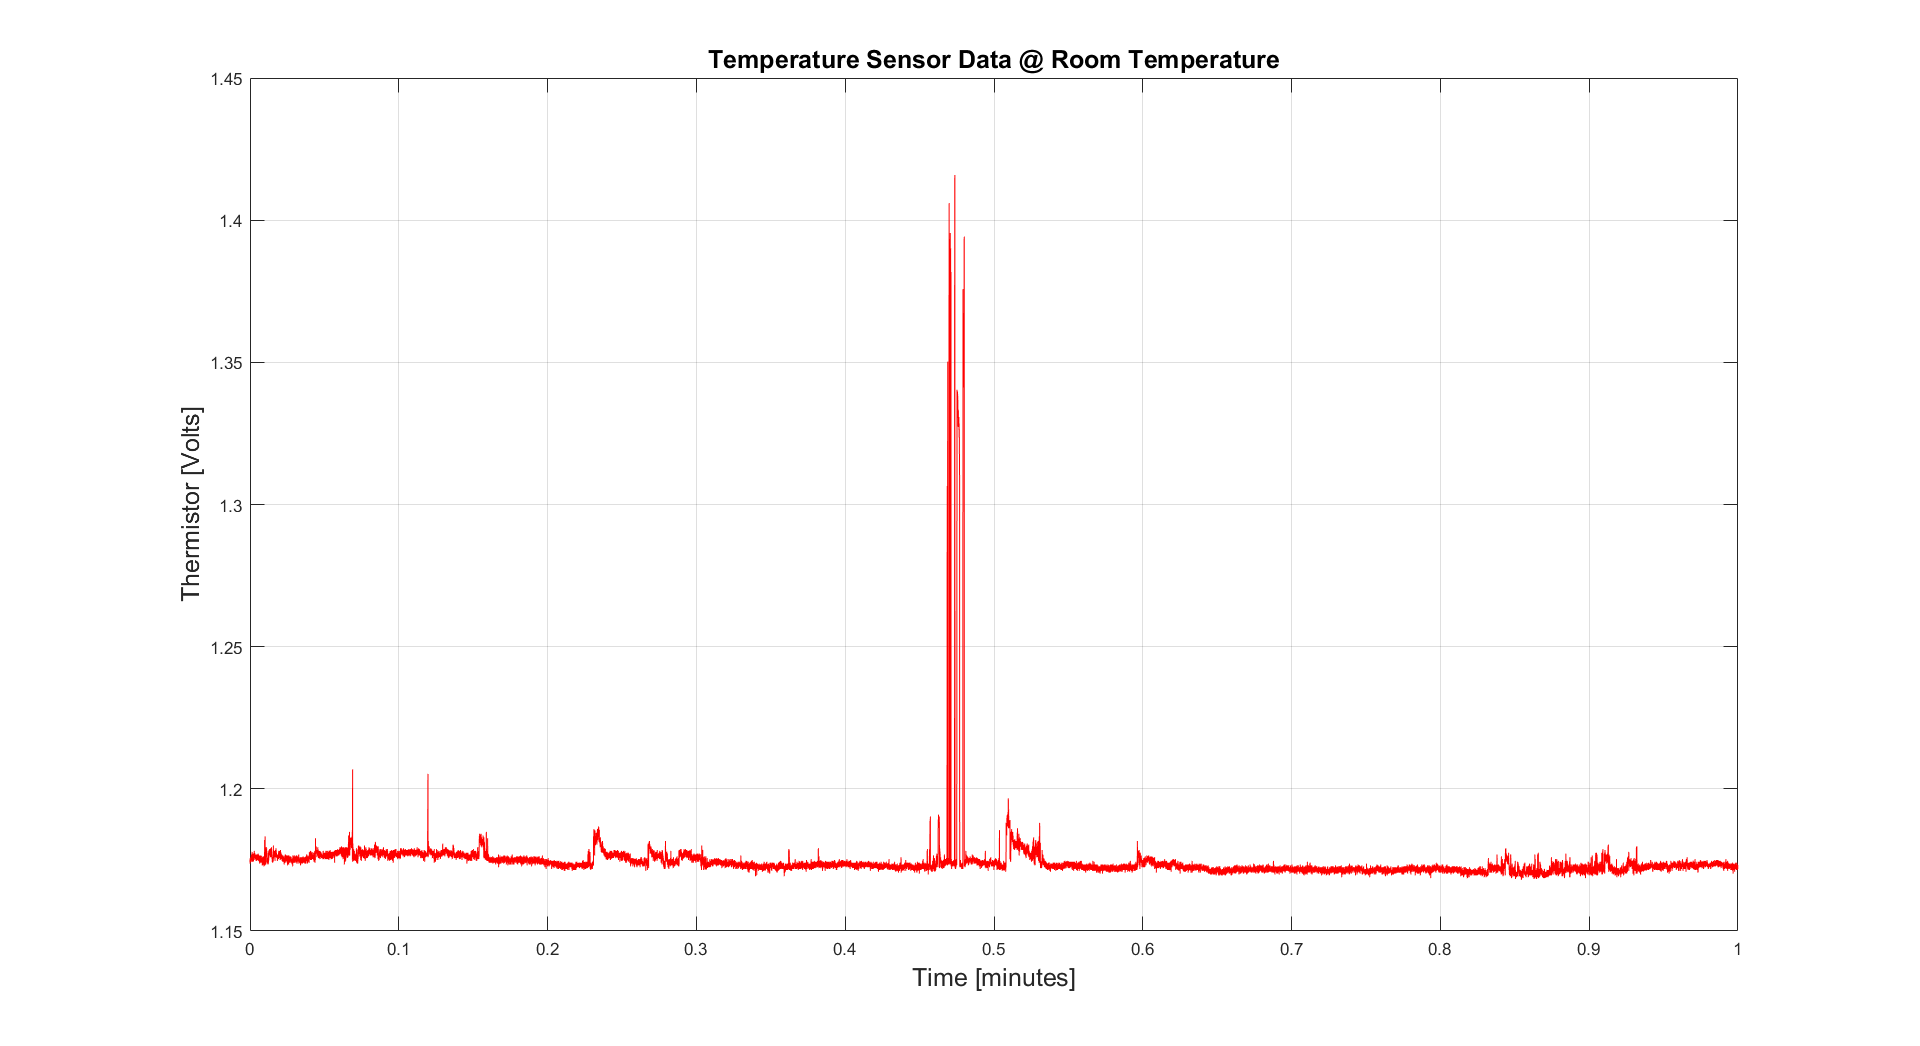
\includegraphics[width=0.985\textwidth]{Lab 2/lab2images/thermistor_volt_roomtemp_1min_plot.png}
    \caption{Thermistor at ambient temperature}
\end{figure}

\begin{figure}[H]
    \centering
    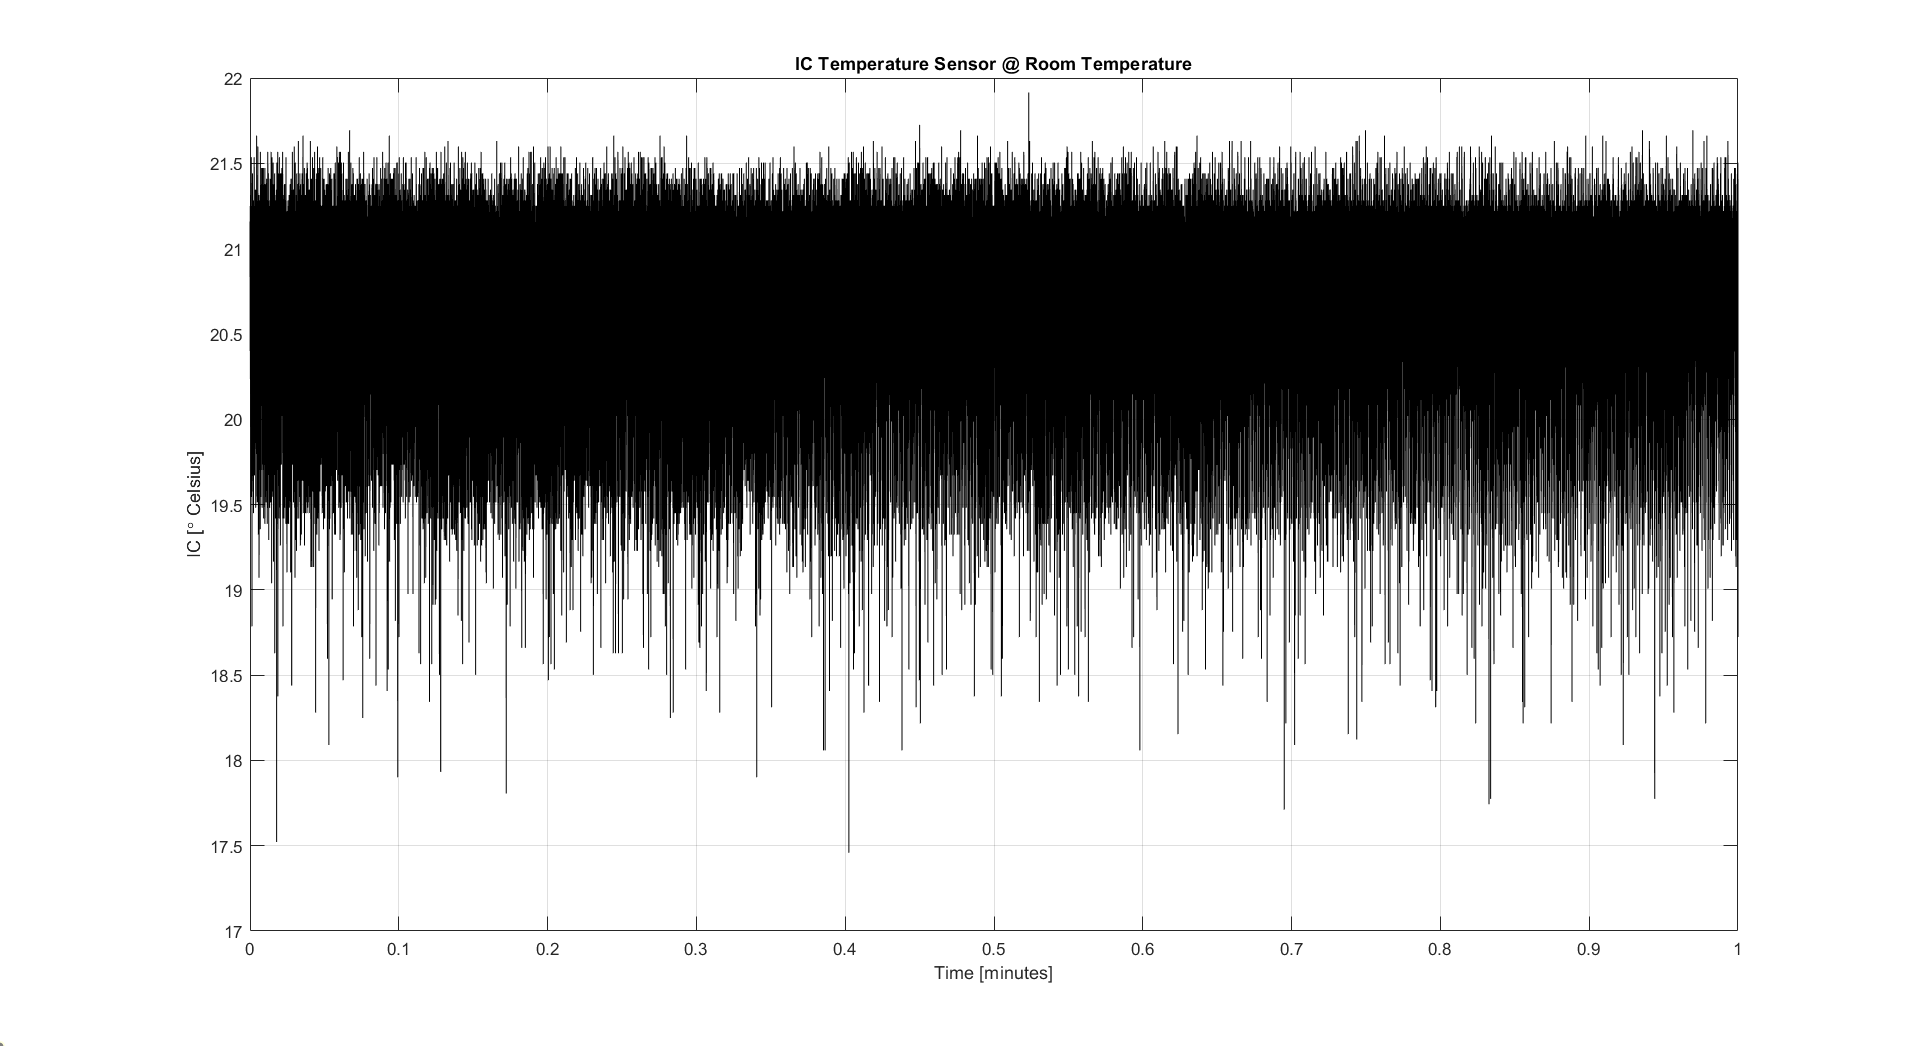
\includegraphics[width=0.985\textwidth]{Lab 2/lab2images/ICTMP36_roomtemp_1min_plot.png}
    \caption{IC TMP36 at ambient temperature}
\end{figure}

\begin{figure}[H]
    \centering
    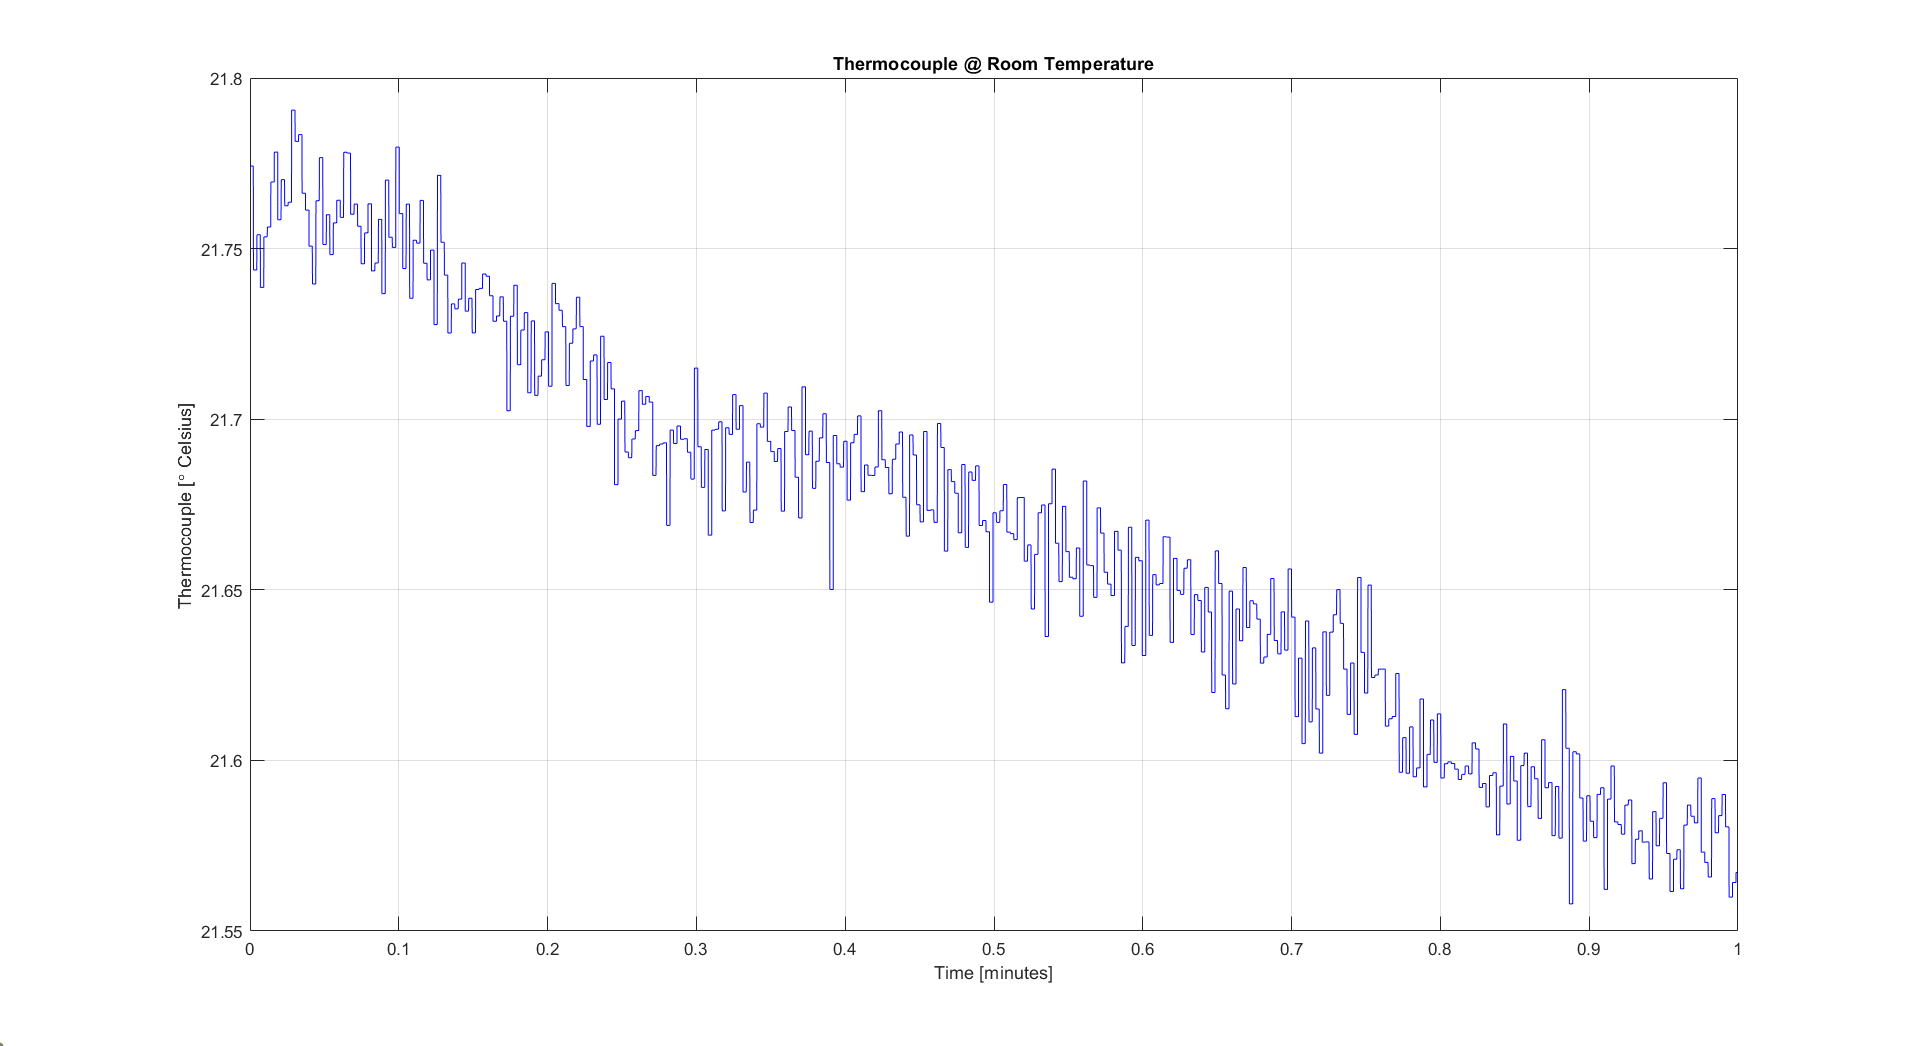
\includegraphics[width=0.985\textwidth]{Lab 2/lab2images/thermocouple_roomtemp_1min_plot.png}
    \caption{Thermocouple at ambient temperature}
\end{figure}

\subsection{Part 2}


\section{Results and Analysis}
(Answer Observation Questions from Part 2)


\section{Conclusion}




\newpage
\thispagestyle{empty}  % Clear header/footer
\begin{center}
	\vspace*{\fill}
	{\Huge Appendices}
	\vspace*{\fill}
\end{center}

% Start appendices
\newpage
\begin{appendices}
\pagestyle{fancy}
\renewcommand{\thefigure}{A\arabic{figure}}
\setcounter{figure}{0}

\section*{Appendix: t-Distribution Tables}
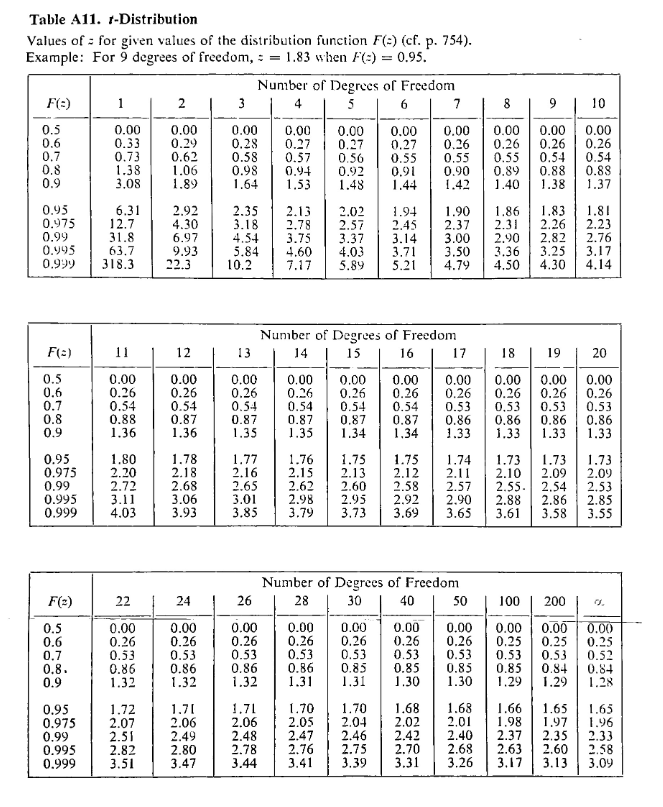
\includegraphics[width=0.95\textwidth]{Lab 1/t_distribution_Table_lecture3.png}
\end{appendices}


\end{document}
